\section{Execise Integration}\label{5_2_gestureConstruction}
%- Recording of gestures --> Kinectstudio --> Making/Train gestures --> Visual gestures builder
The SLS leads the trainee through predefined exercises for slacklining. In development it is important to know that the exercises are defined as \textit{gestures}. The \textit{Kinect for Windows Human Interface Guidelines} describe the term gesture as follows: "\textit{[...] we use the term gesture broadly to mean any form of movement that can be used as an input or interaction to control or influence an application.}"~\cite{MicrosoftHIG2014-mh}.

There are two approaches for creating custom gestures.
The first one is to do heuristics, which means to manually track the position of each joint of the user. Conditions can then be defined according to the action that should happen e.g. if a joint exceed a certain threshold or is in a defined range.
This can be easily used for simple gestures like raising the hand over the head.
For more complex gestures, the developer must have a good understanding about the movement and behaviour of the human body.
Furthermore, environmental factors, like an inappropriate mounting of the Kinect, could exacerbate managing and maintaining the code.
Usually a common developer has not the appropriate expertise of the human body behaviour. Hence, it is recommended to use the Visual gesture builder (VGB) provided by Microsoft for this case.
It uses machine learning to build a database out of pre-recorded clips by the developer.
Afterwards the database can be implemented in an application to track the desired gesture.
The cons of this are the huge file size of the recorded clips that can take very much disk space.
Also tagging keyframes for recorded clips, which should be detected by the application is time consuming. 
On the other hand the tool is simple to use and constructing complex gestures can be easy like described in the next subsection.

%any form of movement that can be used as an input or interaction to control or influence an application. Gestures can take many forms, from simply using your hand to target something on the screen, to specific, learned patterns of movement, to long stretches of continuous movement using the whole body.

\begin{comment}
\subsection{Visual gesture builder}
%look at the data given by the developer via pre recorded clips.
%The more data is provided to the database, the better the detection. konkretisieren
The VGB uses machine learning to build a database out of pre-recorded clips by the developer.
Afterwards the database can be implemented in an application to track the defined gesture.

A major advantage is that environmental factors are not as complex to handle as in comparison to heuristics.
For example if the application should cover that the Kinect can be mounted in an inappropriate height, the developer has to consider this in his heuristics.
Managing and maintaining such factors in code can be demanding.

With the VGB the developer just records data with the Kinect in the appropriate height and let the machine learning algorithm learn it.
The cons are the huge file size of the recorded clips which can take very much disk space.
Also tagging keyframes for recorded clips, which should be detected by the application is time consuming. 
On the other hand the tool is simple to use and constructing complex gestures can be easy like described in the next subsection.
\end{comment}

\subsection{Workflow for Building Gestures}
The workflow for creating a gesture follows a general routine (Figure~\ref{fig:5_3_gestureCreation}). 
At first the gesture has to be recorded via \textit{KinectStudio}. This is a tool provided by Microsoft for monitoring and recording clips of the Kinect streams. Before inserting the clip into the VGB a new project has to be created. Therefore the developer first selects the body parts that are necessary for the gesture. After that an indicator has to be defined, i.e. if it is a discrete or continuous gesture. Discrete gestures underlay a conditional check in which the application determines if a certain gesture is currently performed or not. It provides a confidence value that compares the correctness of the persons execution regarding the gestures in the database. This is the majority usage for gesture tracking like e.g. raising the hand or lifting a leg. A continuous gesture however means that its progress can be measured instead of the confidence. Usually multiple small gestures are combined to an entire gesture, for which the progress is essential. This could be for example a golf swing or switching the standing leg~\cite{MicrosoftVGB}.

After the project creation the recordings can be inserted as training data. The developer has to describe a starting as well as an end point of the gesture by tagging the clips. When finished, a gesture database file can be built. For testing reasons it can be analysed via a live preview or with other recorded clips in a separate analysis area. If the testing results are not satisfying, the developer can record and add more clips or adjust the tags of existing clips. Lastly, after the testing phase the gesture database file can be implemented in the application for gesture detection. %The structuring of the application architecture is part of the next section.
\begin{figure}[htb]
	\centering
	\begin{minipage}[t]{1\linewidth}
		\centering
		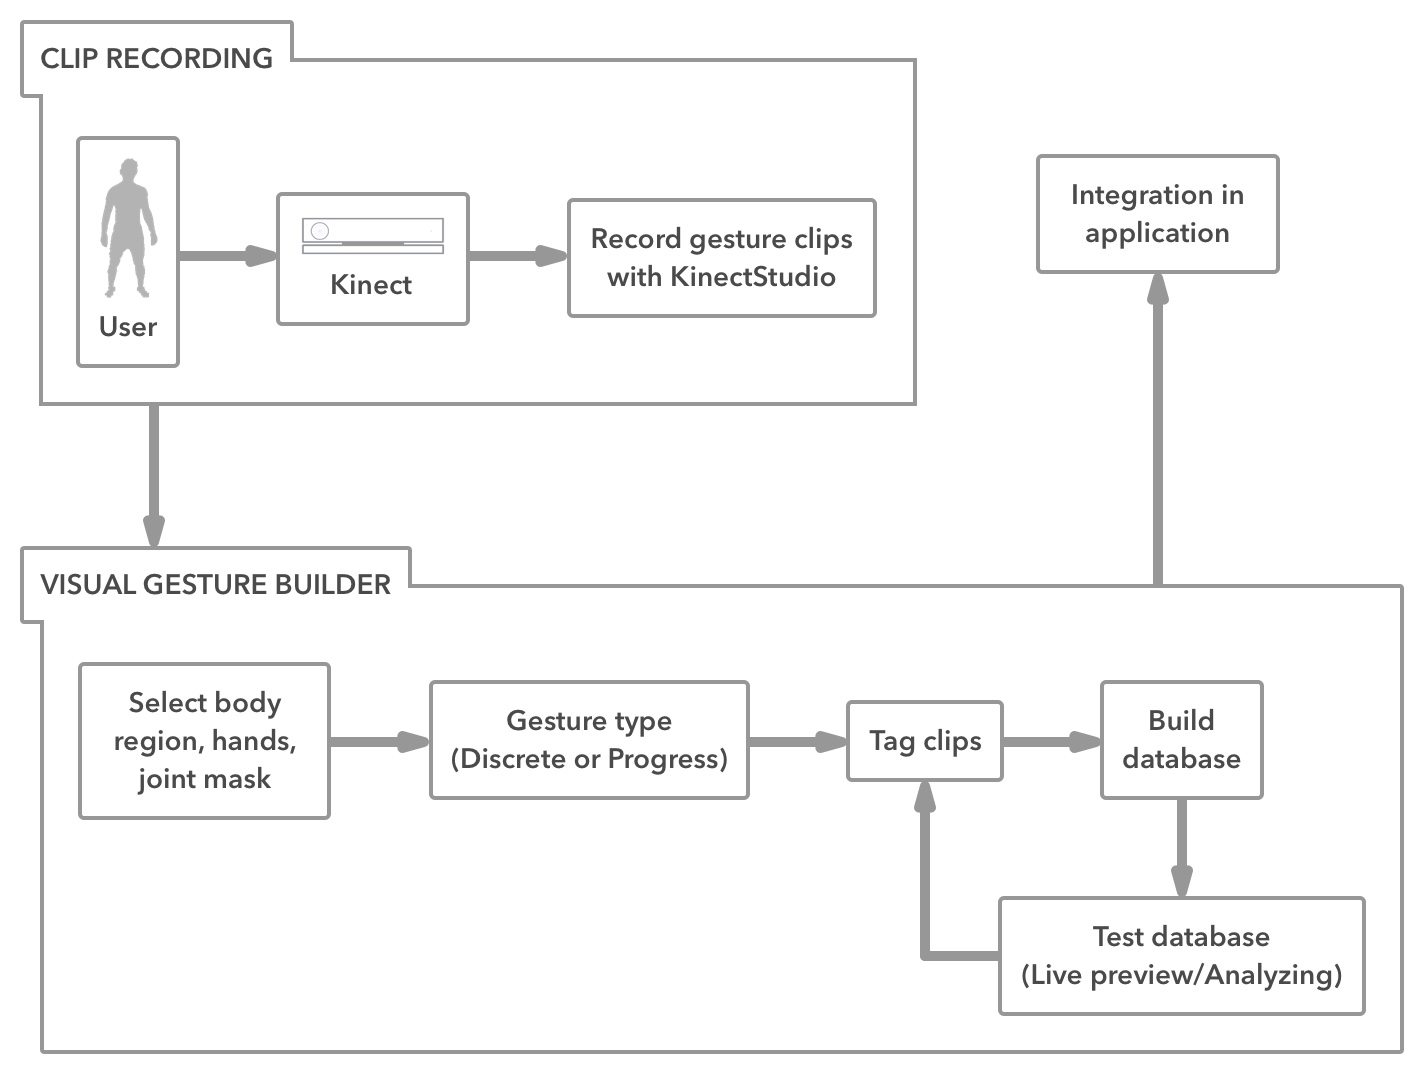
\includegraphics[width=1\linewidth]{Pictures/5_3_gestureCreation}
		\caption{Workflow of creating a gesture database}
		\label{fig:5_3_gestureCreation}
	\end{minipage}
\end{figure}
